\section{Experimental Results}
Two experiments were conducted using the different EAs mentioned in the previous section. The created EAs were tested in the EvoMan Framework \cite{defranca2020evoman} against three different enemies, the \emph{Airman}, the \emph{Metalman}, and the \emph{Quickman}.\par

Each EA runs $10\text{ times}$ for each enemy, while the best individual of every run is being tested $5\text{ times}$. The best individual is selected based on the highest individual gain (equation \ref{gain}) among all generations.\par

In order to evaluate the EAs, two kinds of plots were created. The line plots represent the average of mean and maximum fitness (equation \ref{fitness}) of each generation and their standard deviations, while the box plots depict the individual gain of the best individuals arising from each $training\_run$. Each individual is tested for accuracy reasons $5\text{ times}$, and the gain represented in the plot is the mean of those five $testing$ runs.\par

The three Figures depict the fitness and gain values of the agent that is controlled by the two EAs in the fight against three different enemies.
In the first fight, depicted in \textbf{Figure \ref{fig:enemy2}}, it can be seen that the average fitness of EA2 is slightly poorer compared to EA1. Moreover, the individual gain of EA2 has a higher variance than EA1. 
In the fight against the Metalman enemy, the fitness performance did not differ significantly between both algorithms. As in the fight depicted in \textbf{Figure \ref{fig:enemy5}}, the individual gain of EA1 is much more concentrated than for EA2. 
The fight against Quickman, \textbf{Figure \ref{fig:enemy8}}, shows the greatest differences between the fitness values. The EA2 shows a worse fitness performance than the EA1 with a higher standard deviation. Also, the box plot emphasizes a high range in individual gain for EA2 in comparison to EA1. Furthermore, some agents controlled by EA2 had a negative individual gain. \par
\intextsep

\begin{figure}[H]%
	\centering
	\subfloat{{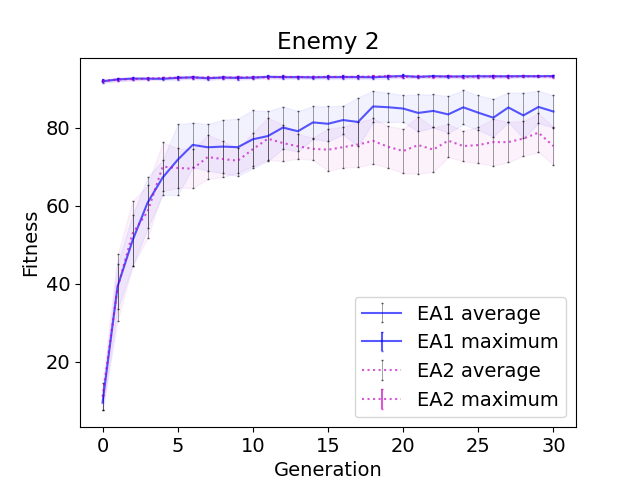
\includegraphics[scale=0.23]{Assets/Enemy2_LinePlot_2.png} }}%
	\qquad
	\subfloat{{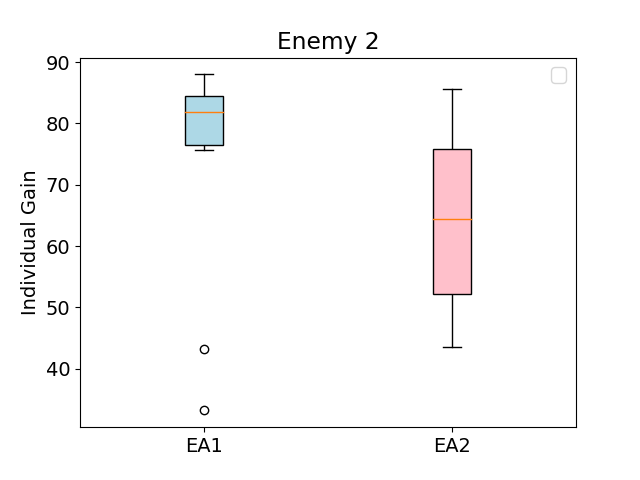
\includegraphics[scale=0.23]{Assets/Enemy2_Boxplot_2.png} }}%
	\caption{Airman Enemy}
	\label{fig:enemy2}
\end{figure}
\begin{figure}[H]%
	\centering
	\subfloat{{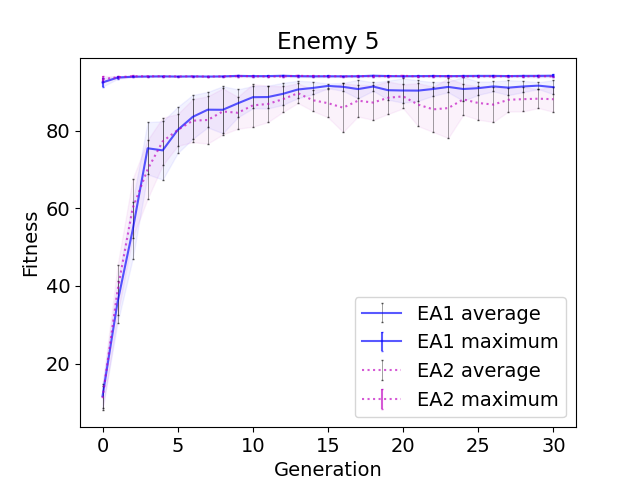
\includegraphics[scale=0.23]{Assets/Enemy5_LinePlot_2.png} }}%
	\qquad
	\subfloat{{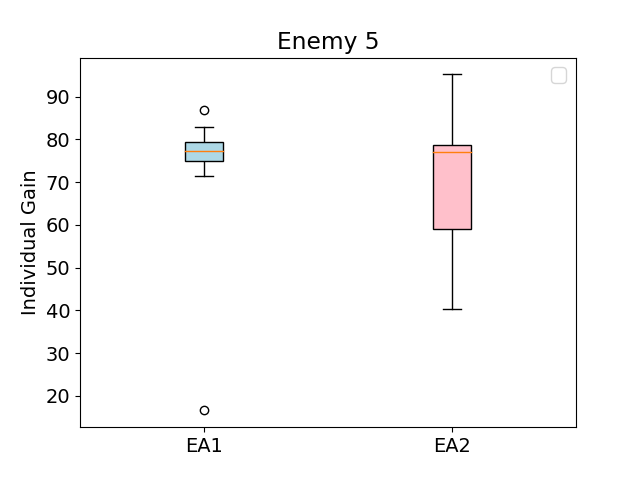
\includegraphics[scale=0.23]{Assets/Enemy5_Boxplot_2.png} }}%
	\caption{Metalman Enemy}
	\label{fig:enemy5}
\end{figure}
\begin{figure}[H]%
	\centering
	\subfloat{{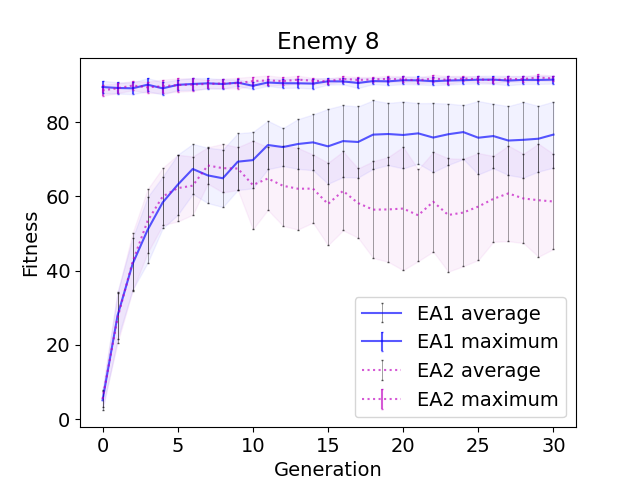
\includegraphics[scale=0.23]{Assets/Enemy8_LinePlot_2.png} }}%
	\qquad
	\subfloat{{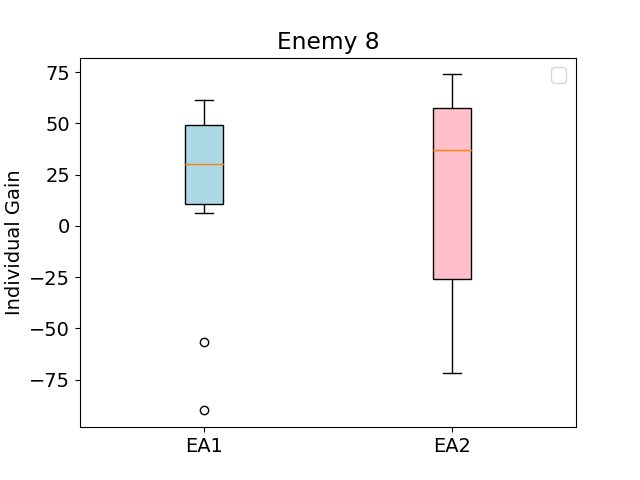
\includegraphics[scale=0.23]{Assets/Enemy8_Boxplot_2.png} }}%
	\caption{Quickman Enemy}
	\label{fig:enemy8}
\end{figure}

